\section{}
    \begin{frame}[allowframebreaks]{Action potential}
        \begin{figure}[H]
            \centering
            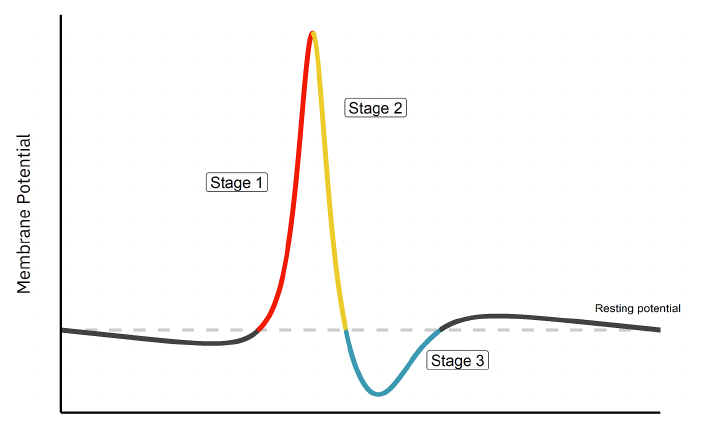
\includegraphics[width=0.5\textwidth]{anatomy/body/nervous_system/neuron/action_potential/wave_form.png}
        \end{figure}
        
        
        \section{Wave form}
            \cite{rueda-2021-a-novel-wave-decomposition-for-oscillatory-signals} propose a wave decomposition method for oscillatory signals based on Frequency Modulated M\"obius (FMM) waves.
            
            \begin{equation}
                W(t)
                =
                A
                \cos
                \Biggl[
                    \beta
                    +
                    2
                    \arctan
                    \Biggl(
                    \omega
                    \tan
                    \Bigl(
                    \frac{t-\alpha}{2}
                    \Bigr)
                    \Biggr)
                    \Biggr]
            \end{equation}
            
            
            \textbf{Neural coding}: Representation with VAE
            \cite{granley-2022-hybrid-neural-autoencoders} Figure 5
            (bottom left shows for each number one njew cluster is formed)
    \end{frame}
    
    \subsection{}
        \begin{frame}[allowframebreaks]{Neuron}
    An exmplary neuron in which Stimuli create an action potential
    \begin{figure}[H]
        \centering
        
\includegraphics[width=0.9\textwidth]{anatomy/body/nervous_system/neuron/neuron_with_action_potential_and_wave_form.png}
    \end{figure}
\end{frame}